\documentclass[11pt]{beamer}

\usetheme[progressbar=frametitle]{metropolis}
\usepackage{appendixnumberbeamer}
\usepackage{pgfpages}
%\setbeameroption{show notes on second screen}



\newcommand{\link}[3][mLightBrown]{\href{#2}{\color{#1}{#3}}}%

\newcommand{\questionslide}[0]{
\section[Your questions]{Time for your questions}
{\setbeamercolor{palette primary}{fg=black, bg=yellow} % bg=peppermint
\begin{frame}[standout]
    \raggedright
  Any questions? \\ \vspace{1cm}
  \raggedleft
  \dots Remember -- this is a safe space! Every question is useful!
\end{frame}
}}

\newenvironment{rcases}
  {\left.\begin{aligned}}
  {\end{aligned}\right\rbrace}

\usepackage{pgfopts}

\newenvironment{rcasesx}
  {\left.\begin{aligned}}
  {\end{aligned}\right.}


\setbeamercolor{block title alerted}{%
    use={block title, alerted text},
    bg=yellow,
    fg=black
}


\definecolor{peppermint}{RGB}{75, 161, 115}

\setbeamercolor{alerted text}{fg=peppermint , bg= black}

\usepackage{booktabs}
\usepackage[scale=2]{ccicons}

\usepackage{pgfplots}
\usepgfplotslibrary{dateplot}

\makeatletter 
\def\beamer@framenotesbegin{% at beginning of slide
    \usebeamercolor[fg]{normal text}
    \gdef\beamer@noteitems{}% 
    \gdef\beamer@notes{}% 
}
\makeatother


\usepackage{xspace}
\newcommand{\themename}{\textbf{\textsc{metropolis}}\xspace}

\title{From Counterfactuals to Linear Regression}
\subtitle{Econ 140 Spring 2025, Section 2}
% \date{\today}
\date{}
\author{Jonathan Old}

\institute{ \link{https://docs.google.com/document/d/1aJLqXpJkgN0fKDtEwYge8xHyxrnHQ2PGlsx9xOsmq-Y/}{Syllabus/OH} \hspace{0.2cm} \link{https://bcourses.berkeley.edu/courses/1542035/files/folder/Sections/Jonathan\%20(Sections\%20110\%2C\%20112)}{bCourses}  \hspace{0.2cm} \link{https://jonathanold.github.io/teaching.html}{Website}  \hspace{0.2cm} \link{https://forms.gle/HuV4DZCKyG5nTbVu6}{Feedback form (\textbf{Always open})} \hspace{0.2cm} \link{https://posit.co/downloads/}{RStudio}}
% \titlegraphic{\hfill\includegraphics[height=1.5cm]{logo.pdf}}

\usepackage{hyperref}

\begin{document}

\begin{frame}
    \titlepage
\end{frame}


\begin{frame}{Roadmap}
  \setbeamertemplate{section in toc}[sections numbered]
  \tableofcontents%[hideallsubsections]
\end{frame}




\questionslide



\section{Selection bias}

\begin{frame}{How to think about Selection Bias}
    \begin{figure}
        \centering
        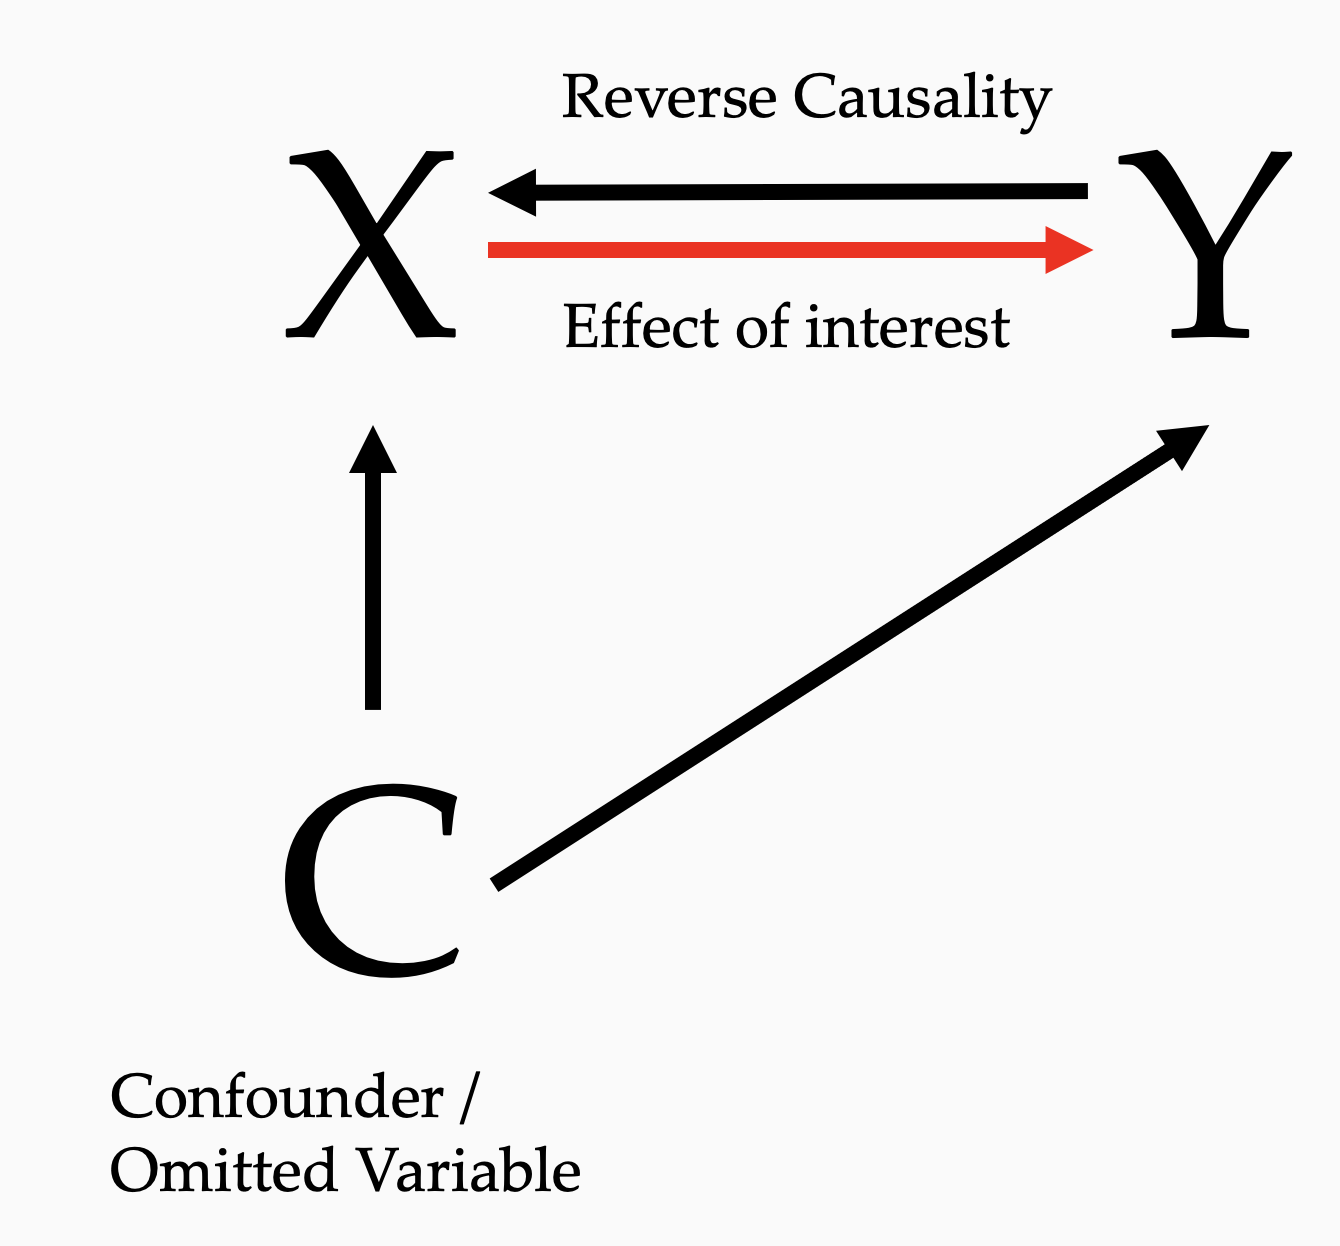
\includegraphics[width=0.5\textwidth]{DAGs/selectionbias.png}
        \caption{Selection bias}
        \label{fig:selectionbias}
    \end{figure}
\end{frame}





\begin{frame}{Dissecting Bad Causal Claims III}

   \begin{alertblock} {\centering \vspace{-1.5ex} \\ Discuss in groups of 2: Why is this statement problematic?  \\ \vspace{-1.5ex} } \end{alertblock}

\begin{figure}[h!t]
    \centering    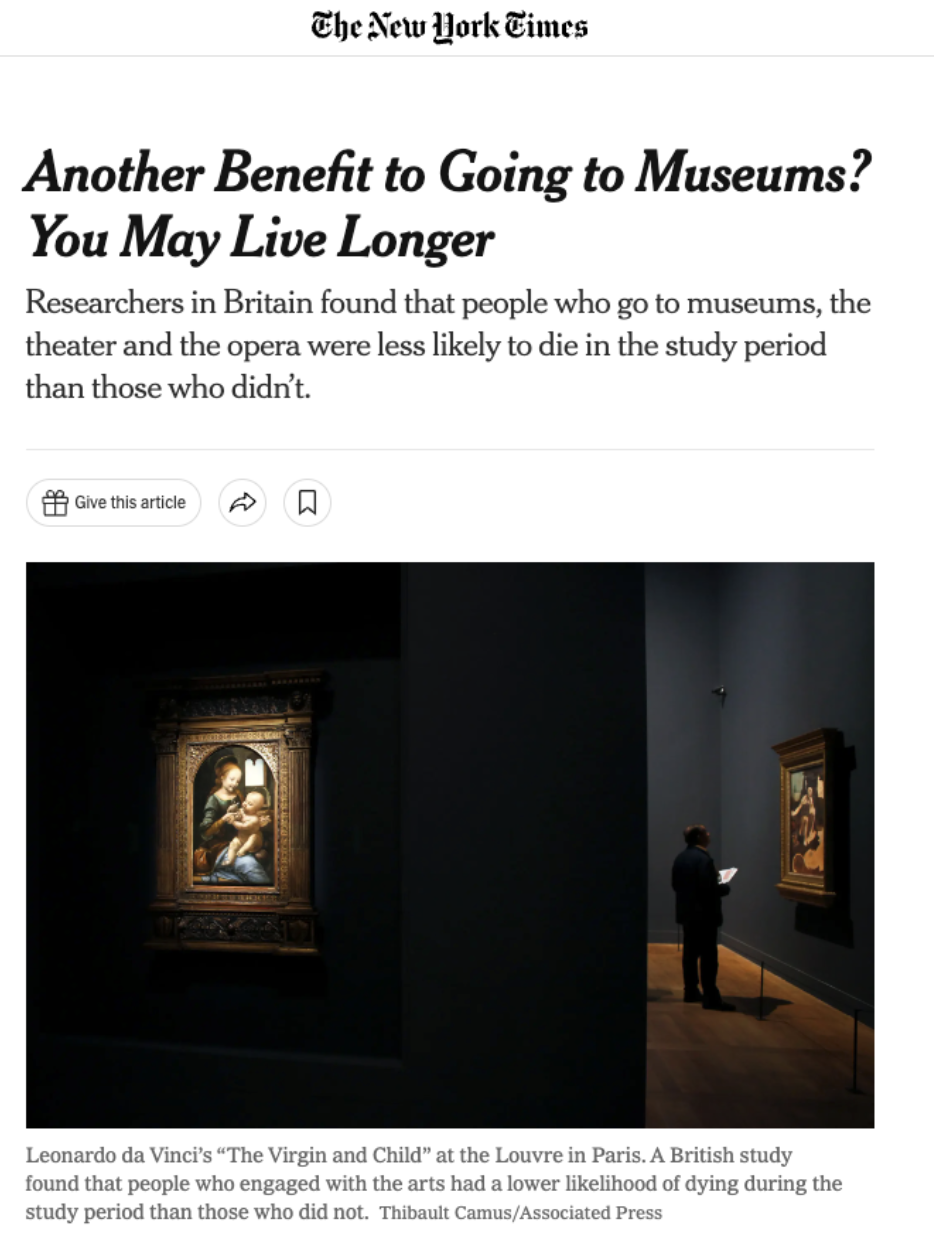
\includegraphics[width=0.42\textwidth]{figures/s1_nytimes.png}
    \caption{Museums and longevity (\href{https://www.nytimes.com/2019/12/22/us/arts-health-effects-ucl-study.html}{Source})}
    \label{fig:museum}
\end{figure}

\end{frame}

















\section{Potential outcomes}
\begin{frame}{Potential outcomes}
    \begin{itemize}
        \item   ``Potential outcomes'' is a framework that can help us \textbf{think through causal claims}: An alternative to math, drawing errors, or thinking things through 
        \item We like to \textbf{write things down} in a rigorous way: Transparent, easy to verify, easy to replicate 
        \item Potential outcomes are {\alert{\textbf{hypothetical}}} outcomes 
        \item Example: Your exam score when you go to all sections vs. when you go to no sections 
        \item Think of potential outcomes as ``\alert{\textbf{parallel universes}}'' 
    \end{itemize}
Our main challenge: We {\color{red}\textbf{\Large{NEVER}}} observe an individual at more than one status at the same time!

\end{frame}







\begin{frame}{Potential outcomes: Notation}
    We write the potential outcomes as:

\begin{align*}
\begin{rcases}
Y_{i0} &= \text{Outcome of individual $i$ with "status" 0} \\
Y_{i1} &= \text{Outcome of individual $i$ with "status" 1} 
\end{rcases}
\begin{rcasesx}
\text{\textbf{\alert{Counterfactual}}} \\
\text{\textbf{\alert{Outcomes}}}
\end{rcasesx}
\end{align*}


Alternative way of writing it: $Y_i(0)$ and $Y_i(1)$

 
    "Status" can be anything
    \begin{itemize}
        \item   Treatment assignment: 0 or 1
        \item Actual treatment: 0 or 1
        \item Drinking expensive whiskey or not
        \item Can also be: Multi-valued (number of children) or continuous (hours studied)
    \end{itemize}


\end{frame}







\begin{frame}{Potential outcomes: Notation}
   
\begin{itemize}
\item We are often interested in the expected (think: average) potential outcome of a group of individuals with a given status. 
\item We write the group behind a conditional sign:\\
$\mathrm{E}\left[\text{Score}_{i0} \mid \text{iPad}_{i}=0\right]$ gives the potential outcome of a group of people that had no iPad, in the "parallel universe" where they don't have an iPad. \
\item Then, $\mathrm{E}\left[\text{Score}_{i1} \mid \text{iPad}_{i}=0\right]$ gives the potental outcome of the same group (that currently have no iPad), in the "parallel universe" where they do have an iPad.
\end{itemize}

\end{frame}





\begin{frame}{Estimating the effect of iPads on grades}

%Note: The official solutions use more general notation. 

Let us start with a difference-in-means comparison: 
\begin{align*}
\Delta &= E[\text{Grade}_i|\text{iPad}_i=1] - E[\text{Grade}_i|\text{iPad}_i=0] \\
& {\color{TolLightBlue}\text{Add and subtract } E[\text{Grade}_i(0)|\text{iPad}_i=1]:} \\
 &=  E[\text{Grade}_i(1)|\text{iPad}_i=1]  {  \color{red}  - E[\text{Grade}_i(0)|\text{iPad}_i=1] \quad + }  \\ 
  &  \qquad {\color{red}E[\text{Grade}_i(0)|\text{iPad}_i=1]} - E[\text{Grade}_i(0)|\text{iPad}_i=0] \\ 
& {\color{TolLightBlue}\text{Use properties of expectations:}} \\ 
   &= E[\text{Grade}_i(1) - \text{Grade}_i(0) | \text{iPad}_i=1] \quad + \\ 
   & \qquad E[\text{Grade}_i(0)|\text{iPad}_i=1] - E[\text{Grade}_i(0)|\text{iPad}_i=0] \\  
& = \onslide<2->{ \text{Treatment effect for group with iPad}  + } \onslide<3->{\text{Selection bias} }
 \end{align*}   
%When we observe the real world,  potential outcomes match  observation:
% For the individuals with an iPad their expected grade is the potential outcome of having an iPad, and for those without an iPad their expected grade is the potential outcome of not having an iPad. So we can rewrite the above as: 
\onslide<4->{
Selection bias: Students with and without iPad have different potential grades: \textbf{even if they both \textit{had} iPads, they would be different}.
}
    
\end{frame}














\begin{frame}{Selection Bias revisited}
    \begin{figure}
        \centering
        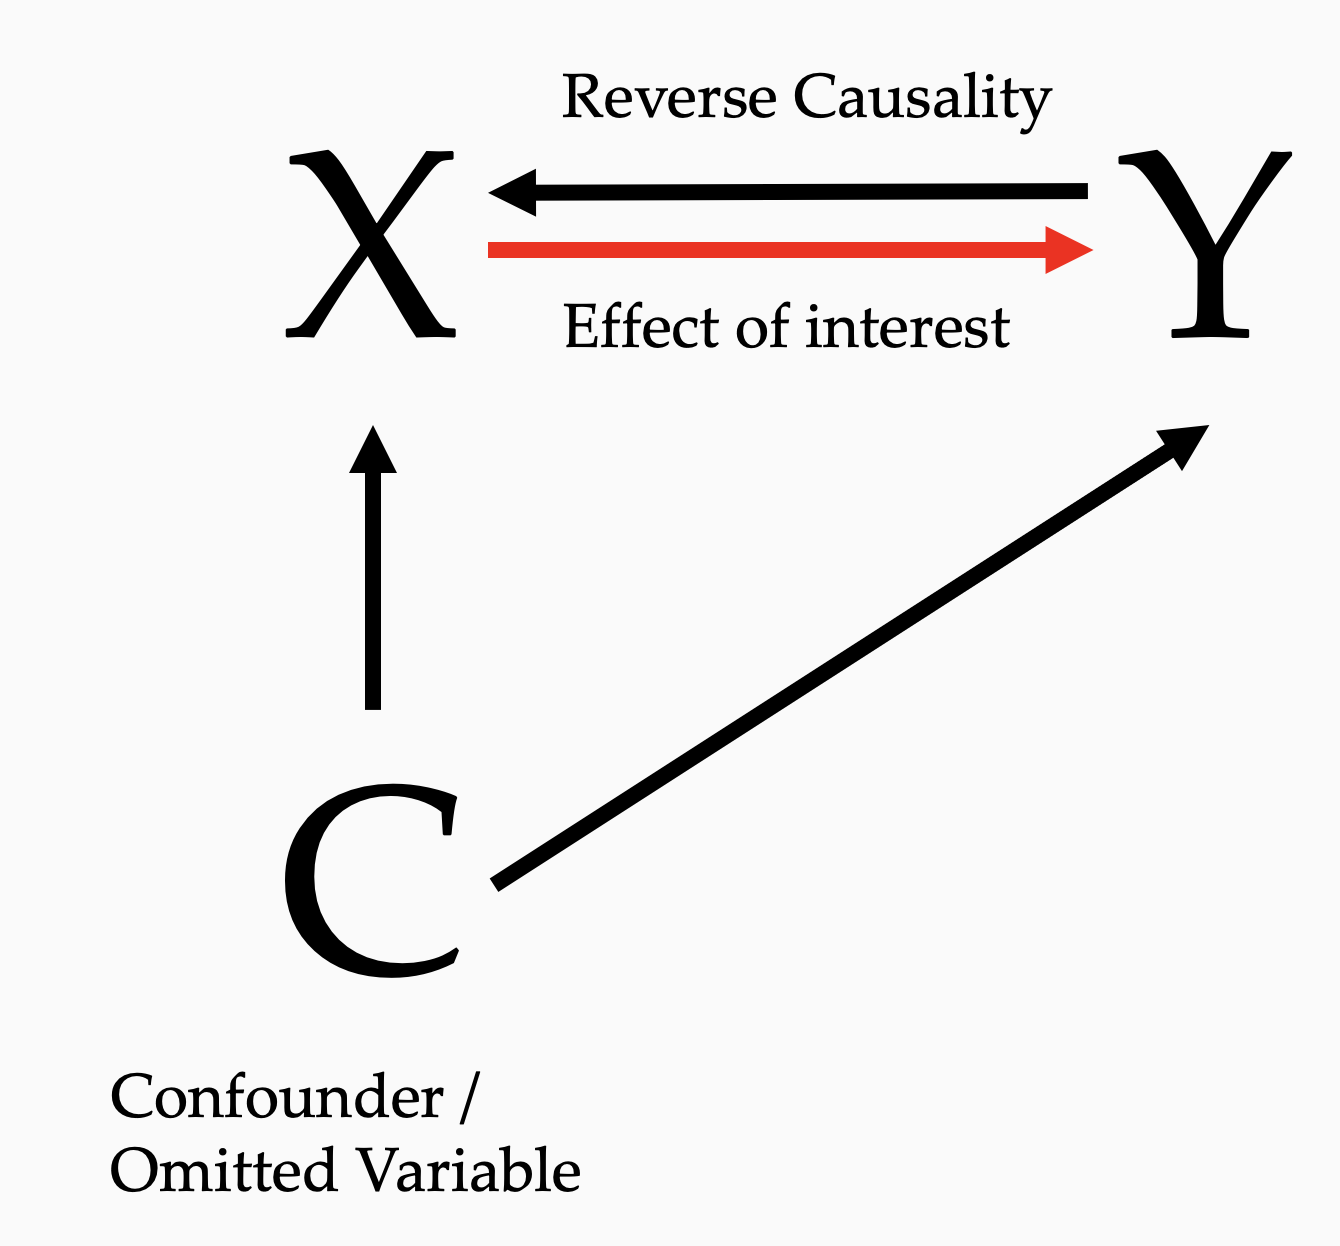
\includegraphics[width=0.5\textwidth]{DAGs/selectionbias.png}
        \caption{Selection bias}
        \label{fig:selectionbias}
    \end{figure}
\end{frame}








\section{RCTs}

\begin{frame}{RCTs solve selection bias}
We had:
\begin{align*}
   \Delta &= E[\text{Grade}_i(1) - \text{Grade}_i(0) | \text{iPad}_i=1] \quad + \\ 
   & \qquad E[\text{Grade}_i(0)|\text{iPad}_i=1] - E[\text{Grade}_i(0)|\text{iPad}_i=0] 
\end{align*}
\vspace{-0.8cm}
\begin{itemize}
    \item The second line was selection bias: The potential grade of individuals with and without iPad is different
    \item If the treatment (iPad) is \textbf{\alert{independent}} of the potential outcomes, then: 
    \begin{align*}
      \text{iPad}_i \perp \left(\text{Grade}_i(1), \text{Grade}_i(0)\right) \\ \Rightarrow E[\text{Grade}_i(0)|\text{iPad}_i=1] = E[\text{Grade}_i(0)|\text{iPad}_i=0]
    \end{align*}

    and selection bias will be zero.


\end{itemize}
\end{frame}


\begin{frame}{Remaining issues with RCTs}

RCTs solve the selection bias problem by \textbf{randomly assigning treatment} to different groups.


   \begin{alertblock} {\centering \vspace{-1.5ex} \\ Discuss in groups: \begin{enumerate} 
   \item Is this the same thing as saying "We drew a random sample from the population?" 
   \item What are some problems with RCTs? \tiny{(ethical/practical/econometric)}  
   \end{enumerate}  \vspace{-1.5ex} } \end{alertblock}
 


\end{frame}



\begin{frame}{RCTs have revolutionized economics}

    \begin{figure}
        \centering
        \href{https://www.npr.org/sections/money/2011/06/08/137041672/the-tuesday-podcast-poor-economics}{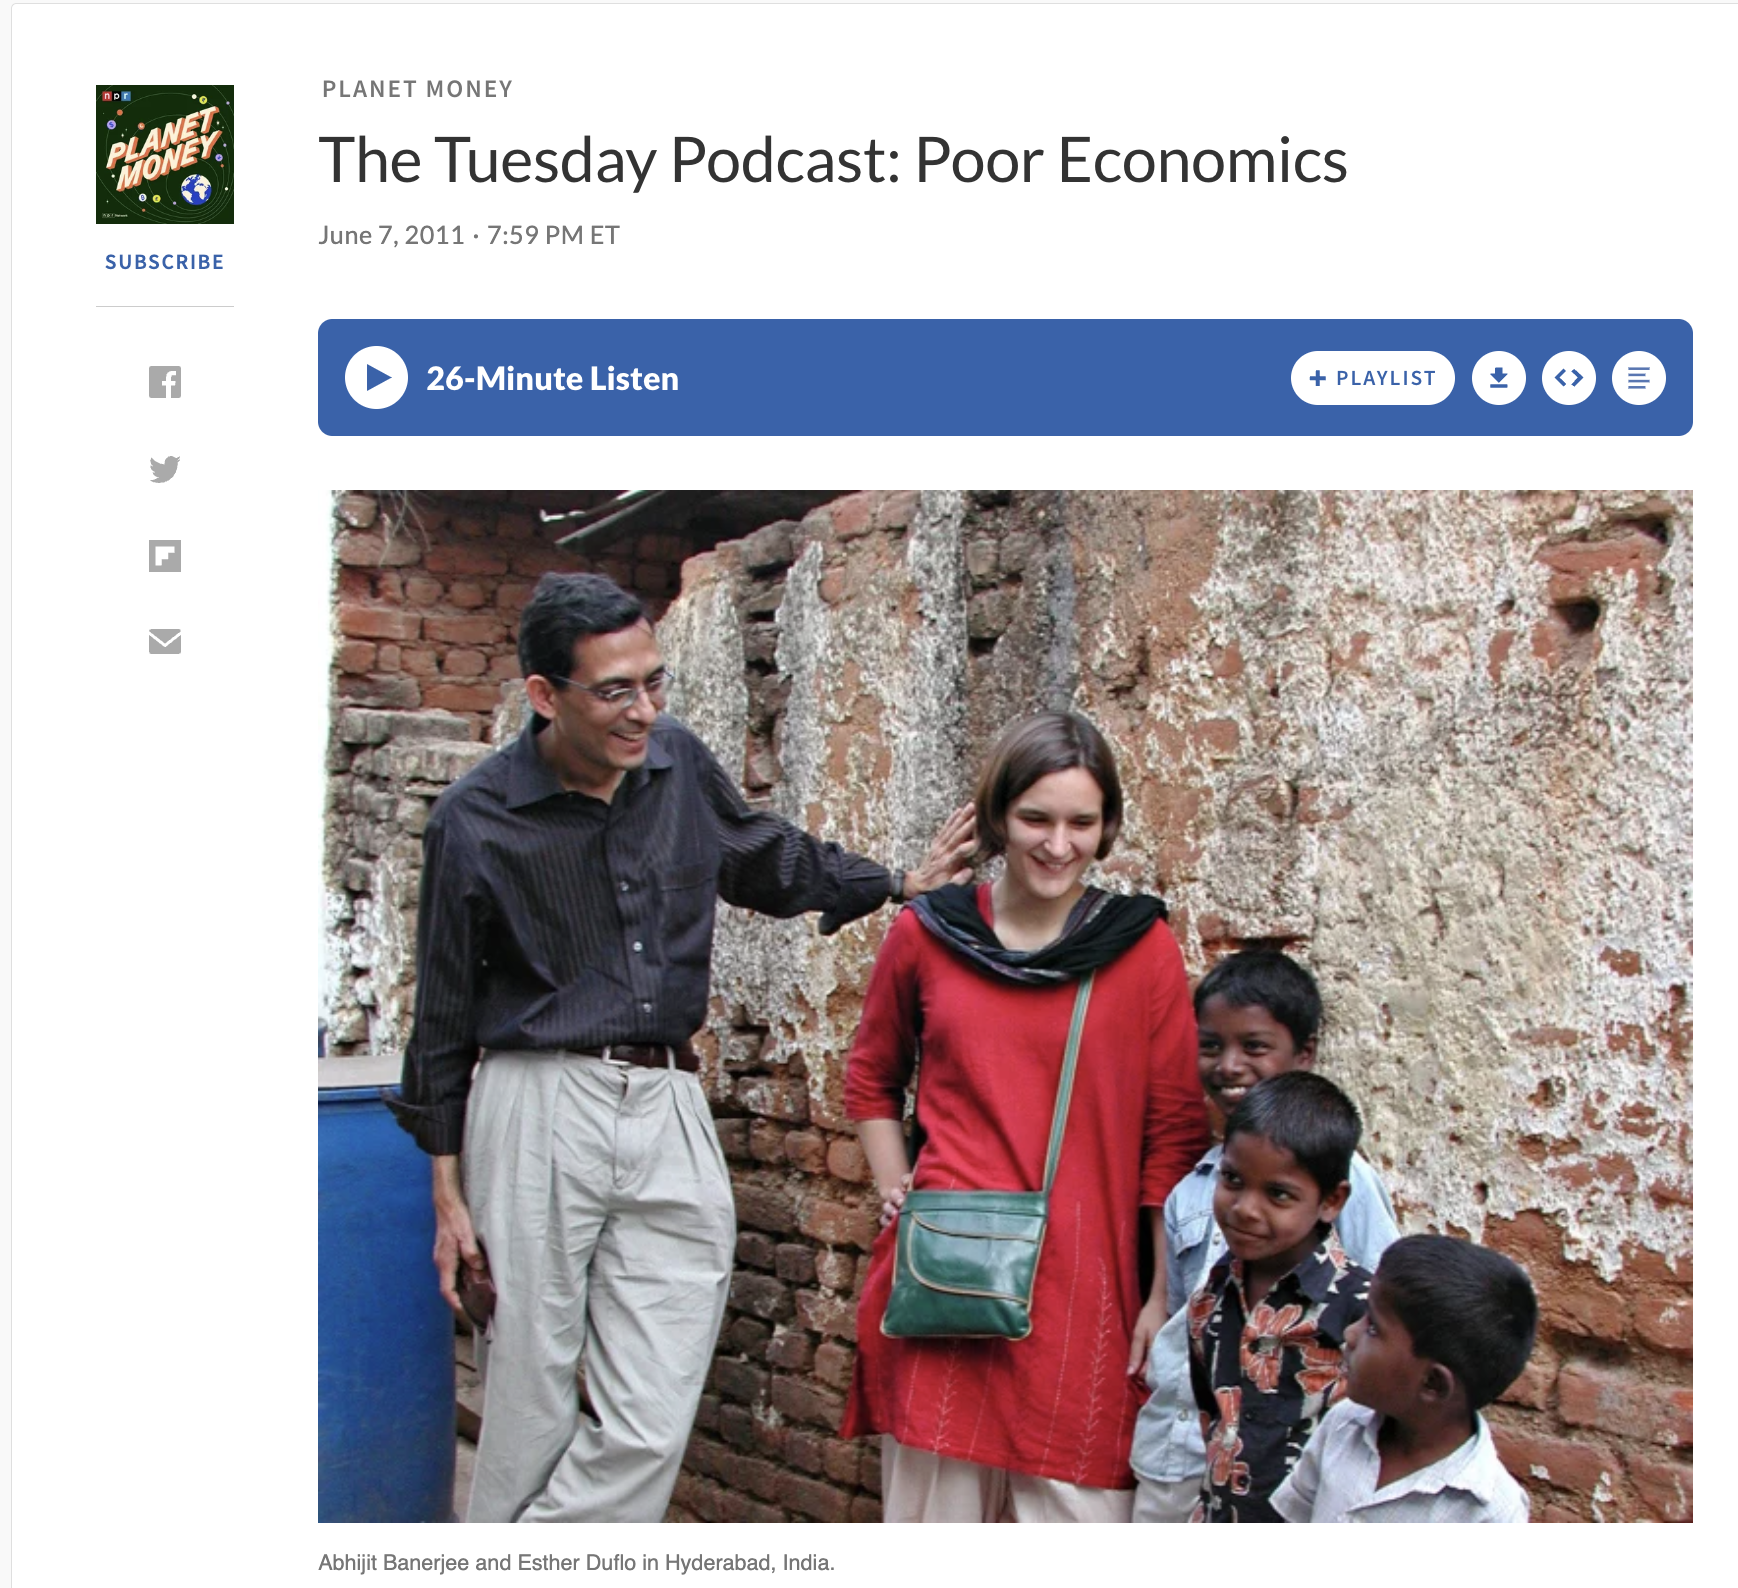
\includegraphics[width=0.7\textwidth]{figures/TeacherPerformancePay/poor_econ.png}}
        \caption{Abhijeet Banerjee and Ester Duflo. (\href{https://www.npr.org/sections/money/2011/06/08/137041672/the-tuesday-podcast-poor-economics}{Source})}
    \end{figure}
\end{frame}



\section[OLS or hypothesis tests: Your choice]{A non-mathematical intro to OLS -- OR: standard errors, t-statistics, and hypothesis tests: What is that all about? \alert{Your choice}}



\begin{frame}{Hypothesis testing}
\begin{itemize}
    \item \alert{Random variables}: Our estimator is a random variable (randomly drawn from population) 
    \item \alert{Standard error}: Random variables have a standard deviation, estimators have standard errors. This quantifies their uncertainty 
    \item \alert{Statistics}: The two keywords are the law of large numbers and the central limit theorem: The sum/mean over many draws from a random variable will be normally distributed
    \item \alert{For hypothesis test}: null and alternative hypothesis. 
    \item Assume the null hypothesis is true, then see \alert{how plausible results are} if it is actually true. 
    \item If they are implausible -- we \alert{reject the null hypothesis}! Otherwise: Fail to reject.
    \end{itemize}
\end{frame}


\begin{frame}{It's all connected}

   \begin{figure}
        \centering
        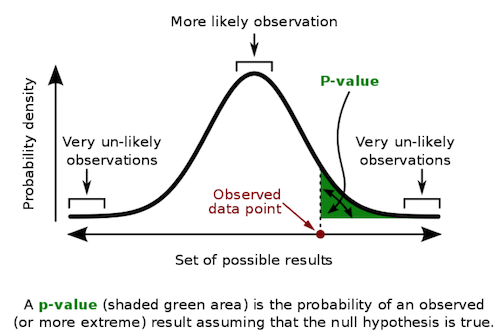
\includegraphics[width=0.8\textwidth]{figures/hypothesis testing/p_value.png}
        
    \end{figure}


\end{frame}

\end{document}
